\section{Solution}

\subsection{Backtracking heuristic}

\begin{frame}{Bellman-like equation}{Heuristic}

%\begin{equation}
%\nonumber
%\hat{x}_{t} = \argmax_{X_{t}} [ f(x_{t} \mid x_{1} , \cdots , x_{t-1}) + \max_{X_{t+1}, \cdots , X_{T}} f(x_{t+1}, \cdots , x_{T} \mid x_{1}, \cdots , x_{t}) ]
%\end{equation}

\centering
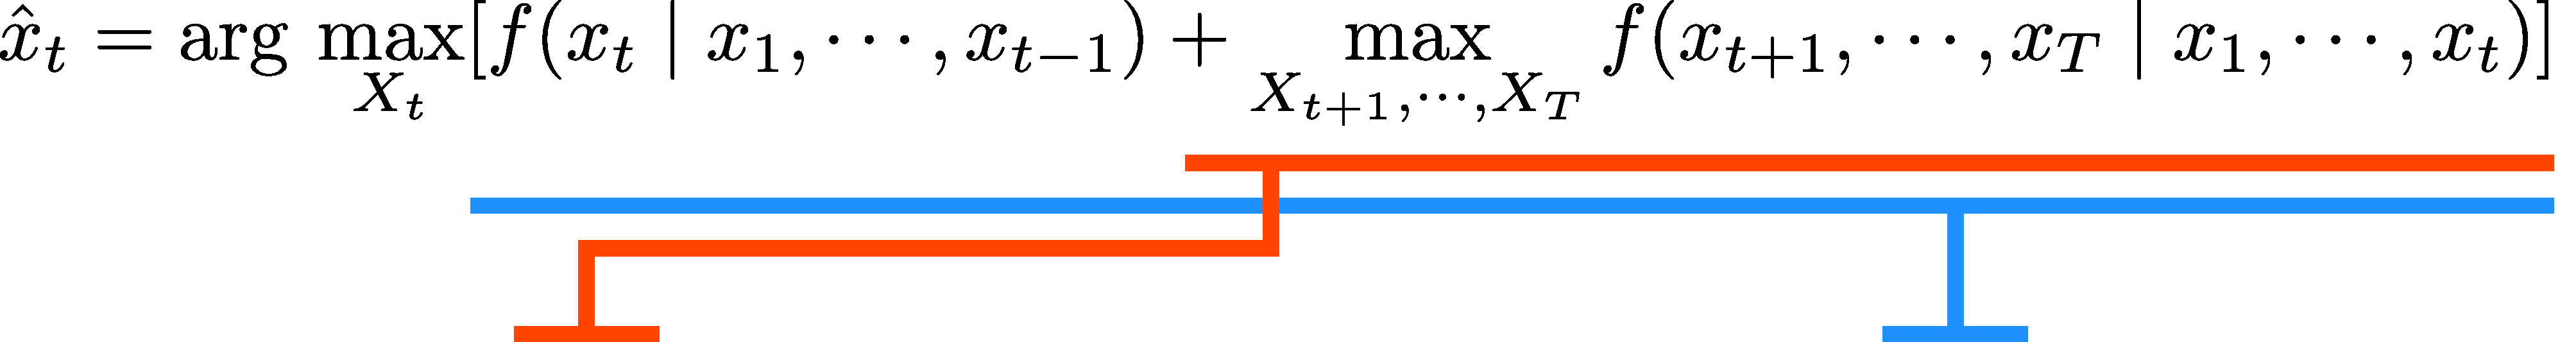
\includegraphics[width = \textwidth]{./figure/arg_equation}

\begin{columns}
\column{0.45\textwidth}
\begin{block}{Maximum future reward}
\begin{figure}
\centering
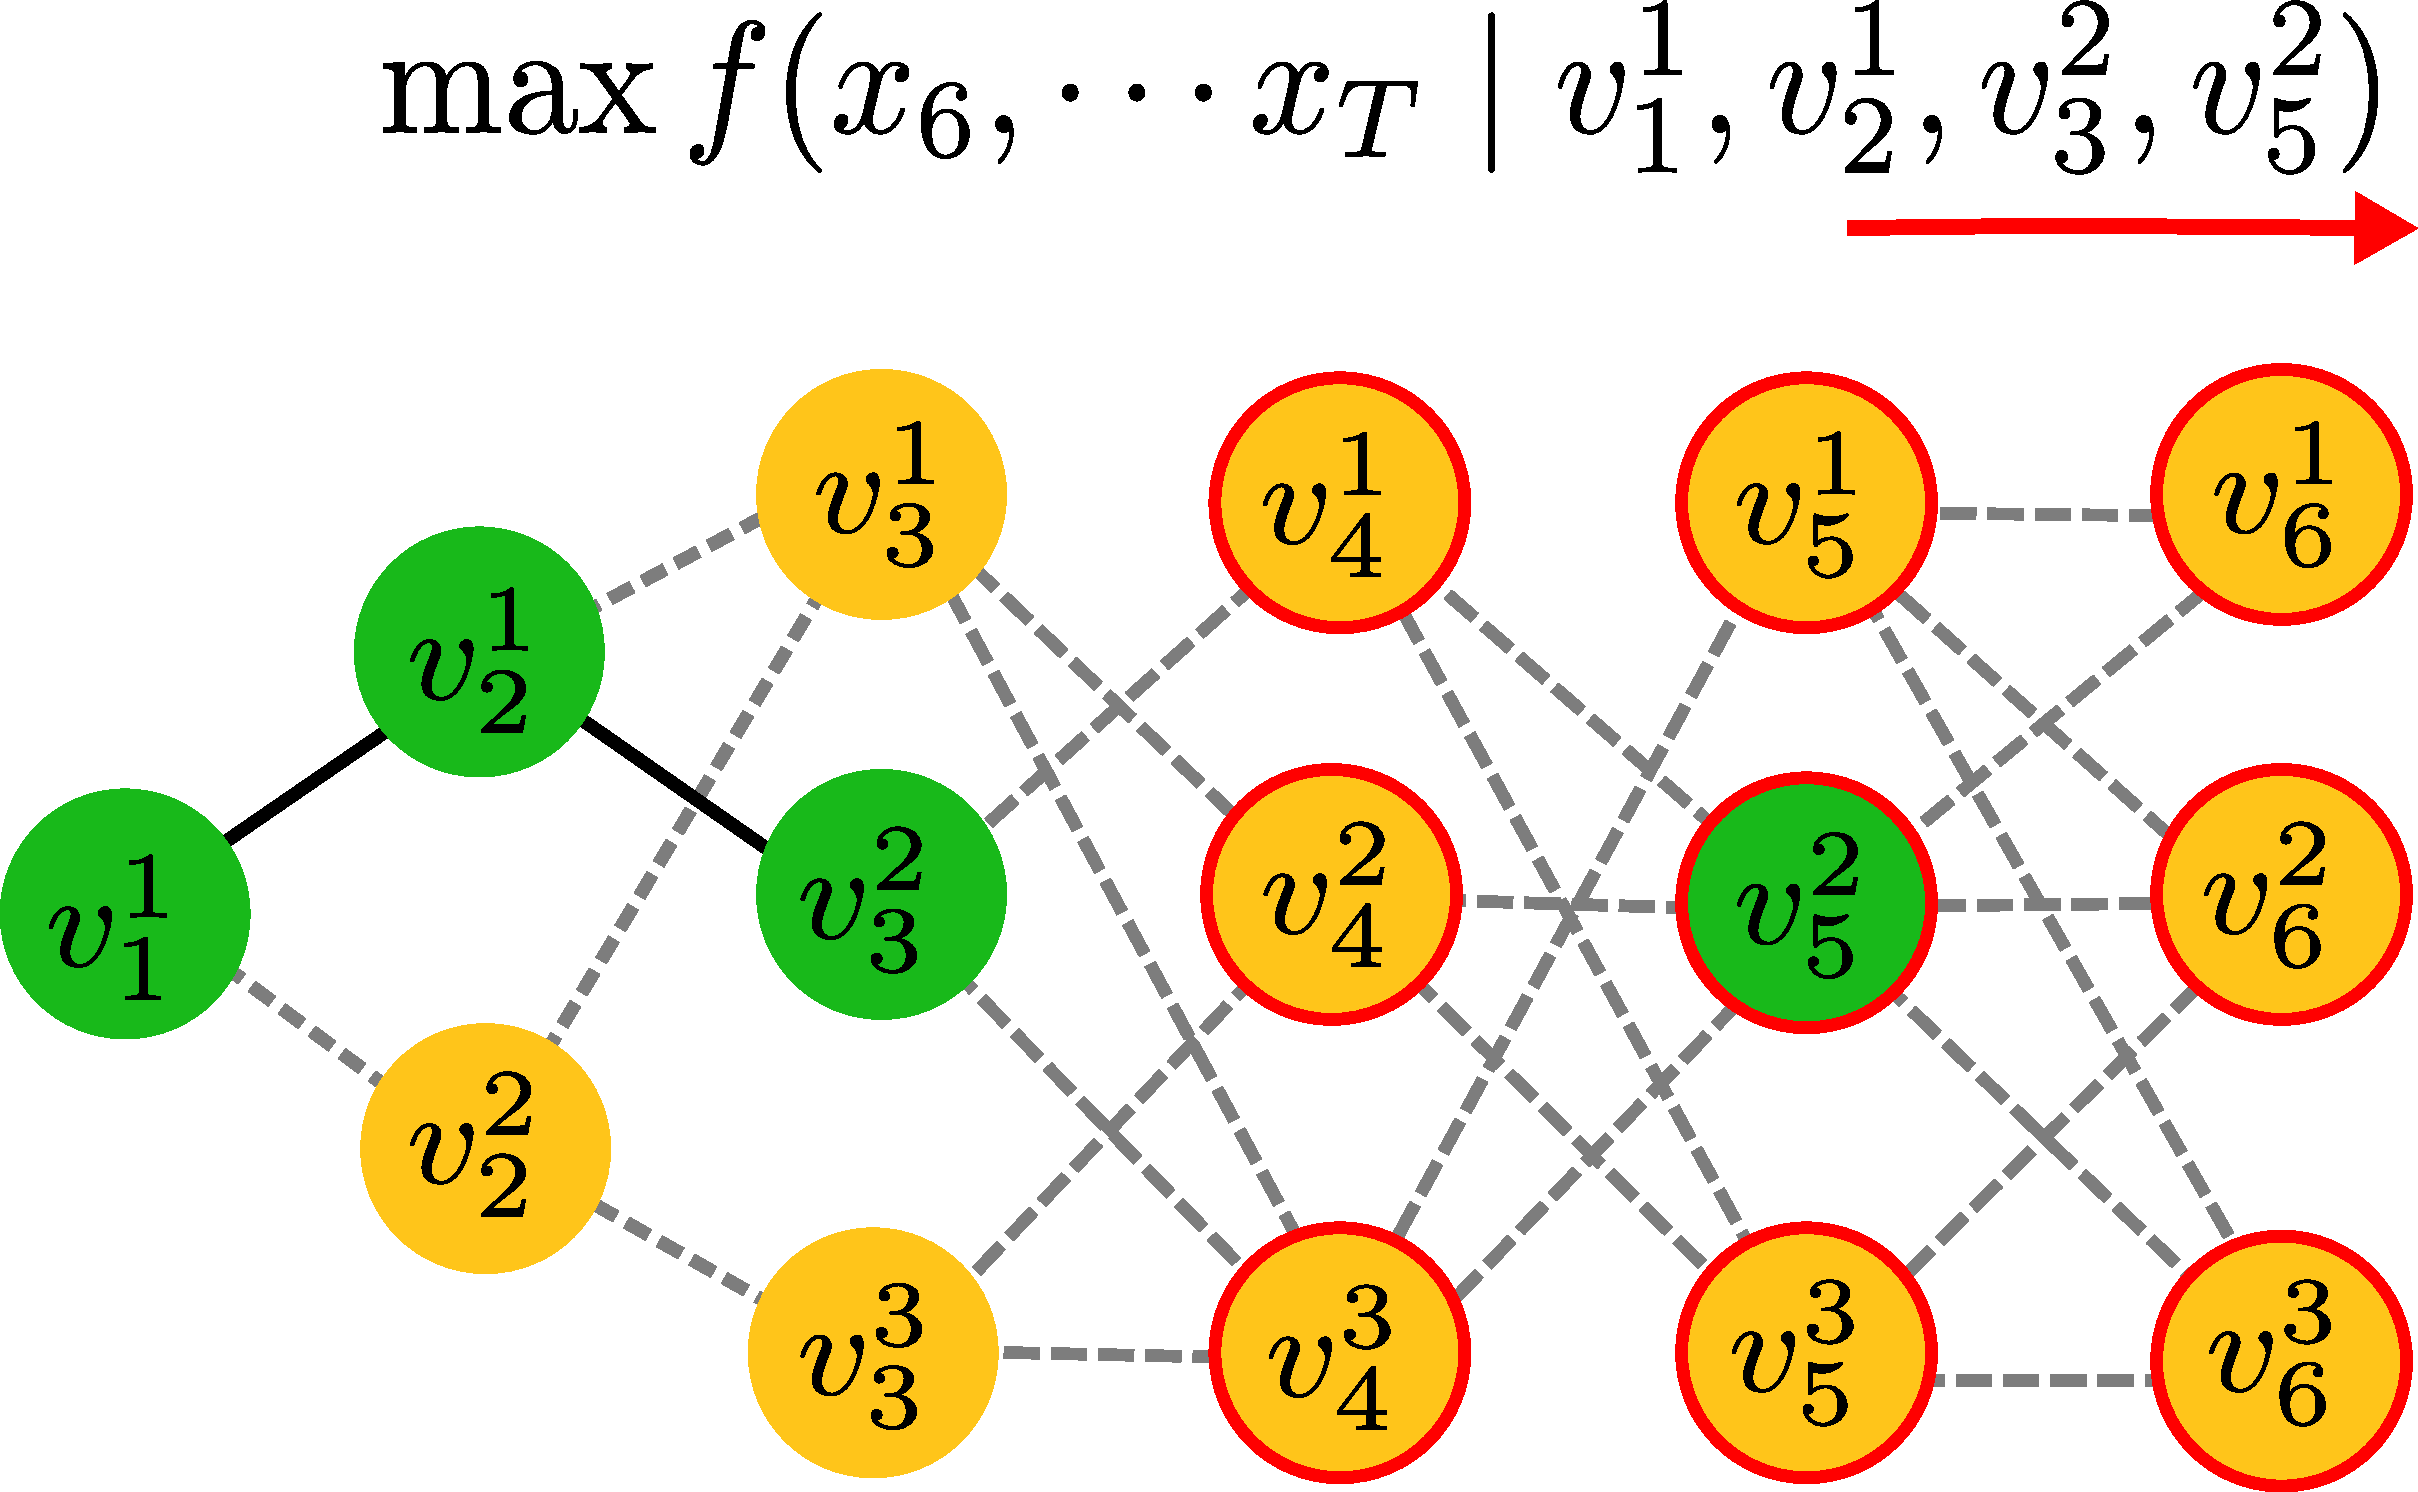
\includegraphics[width = 0.9\textwidth]{./figure/DefineFuncH}
\end{figure}
\end{block}

\column{0.45\textwidth}
\begin{block}{Maximum total reward}
\begin{figure}
\centering
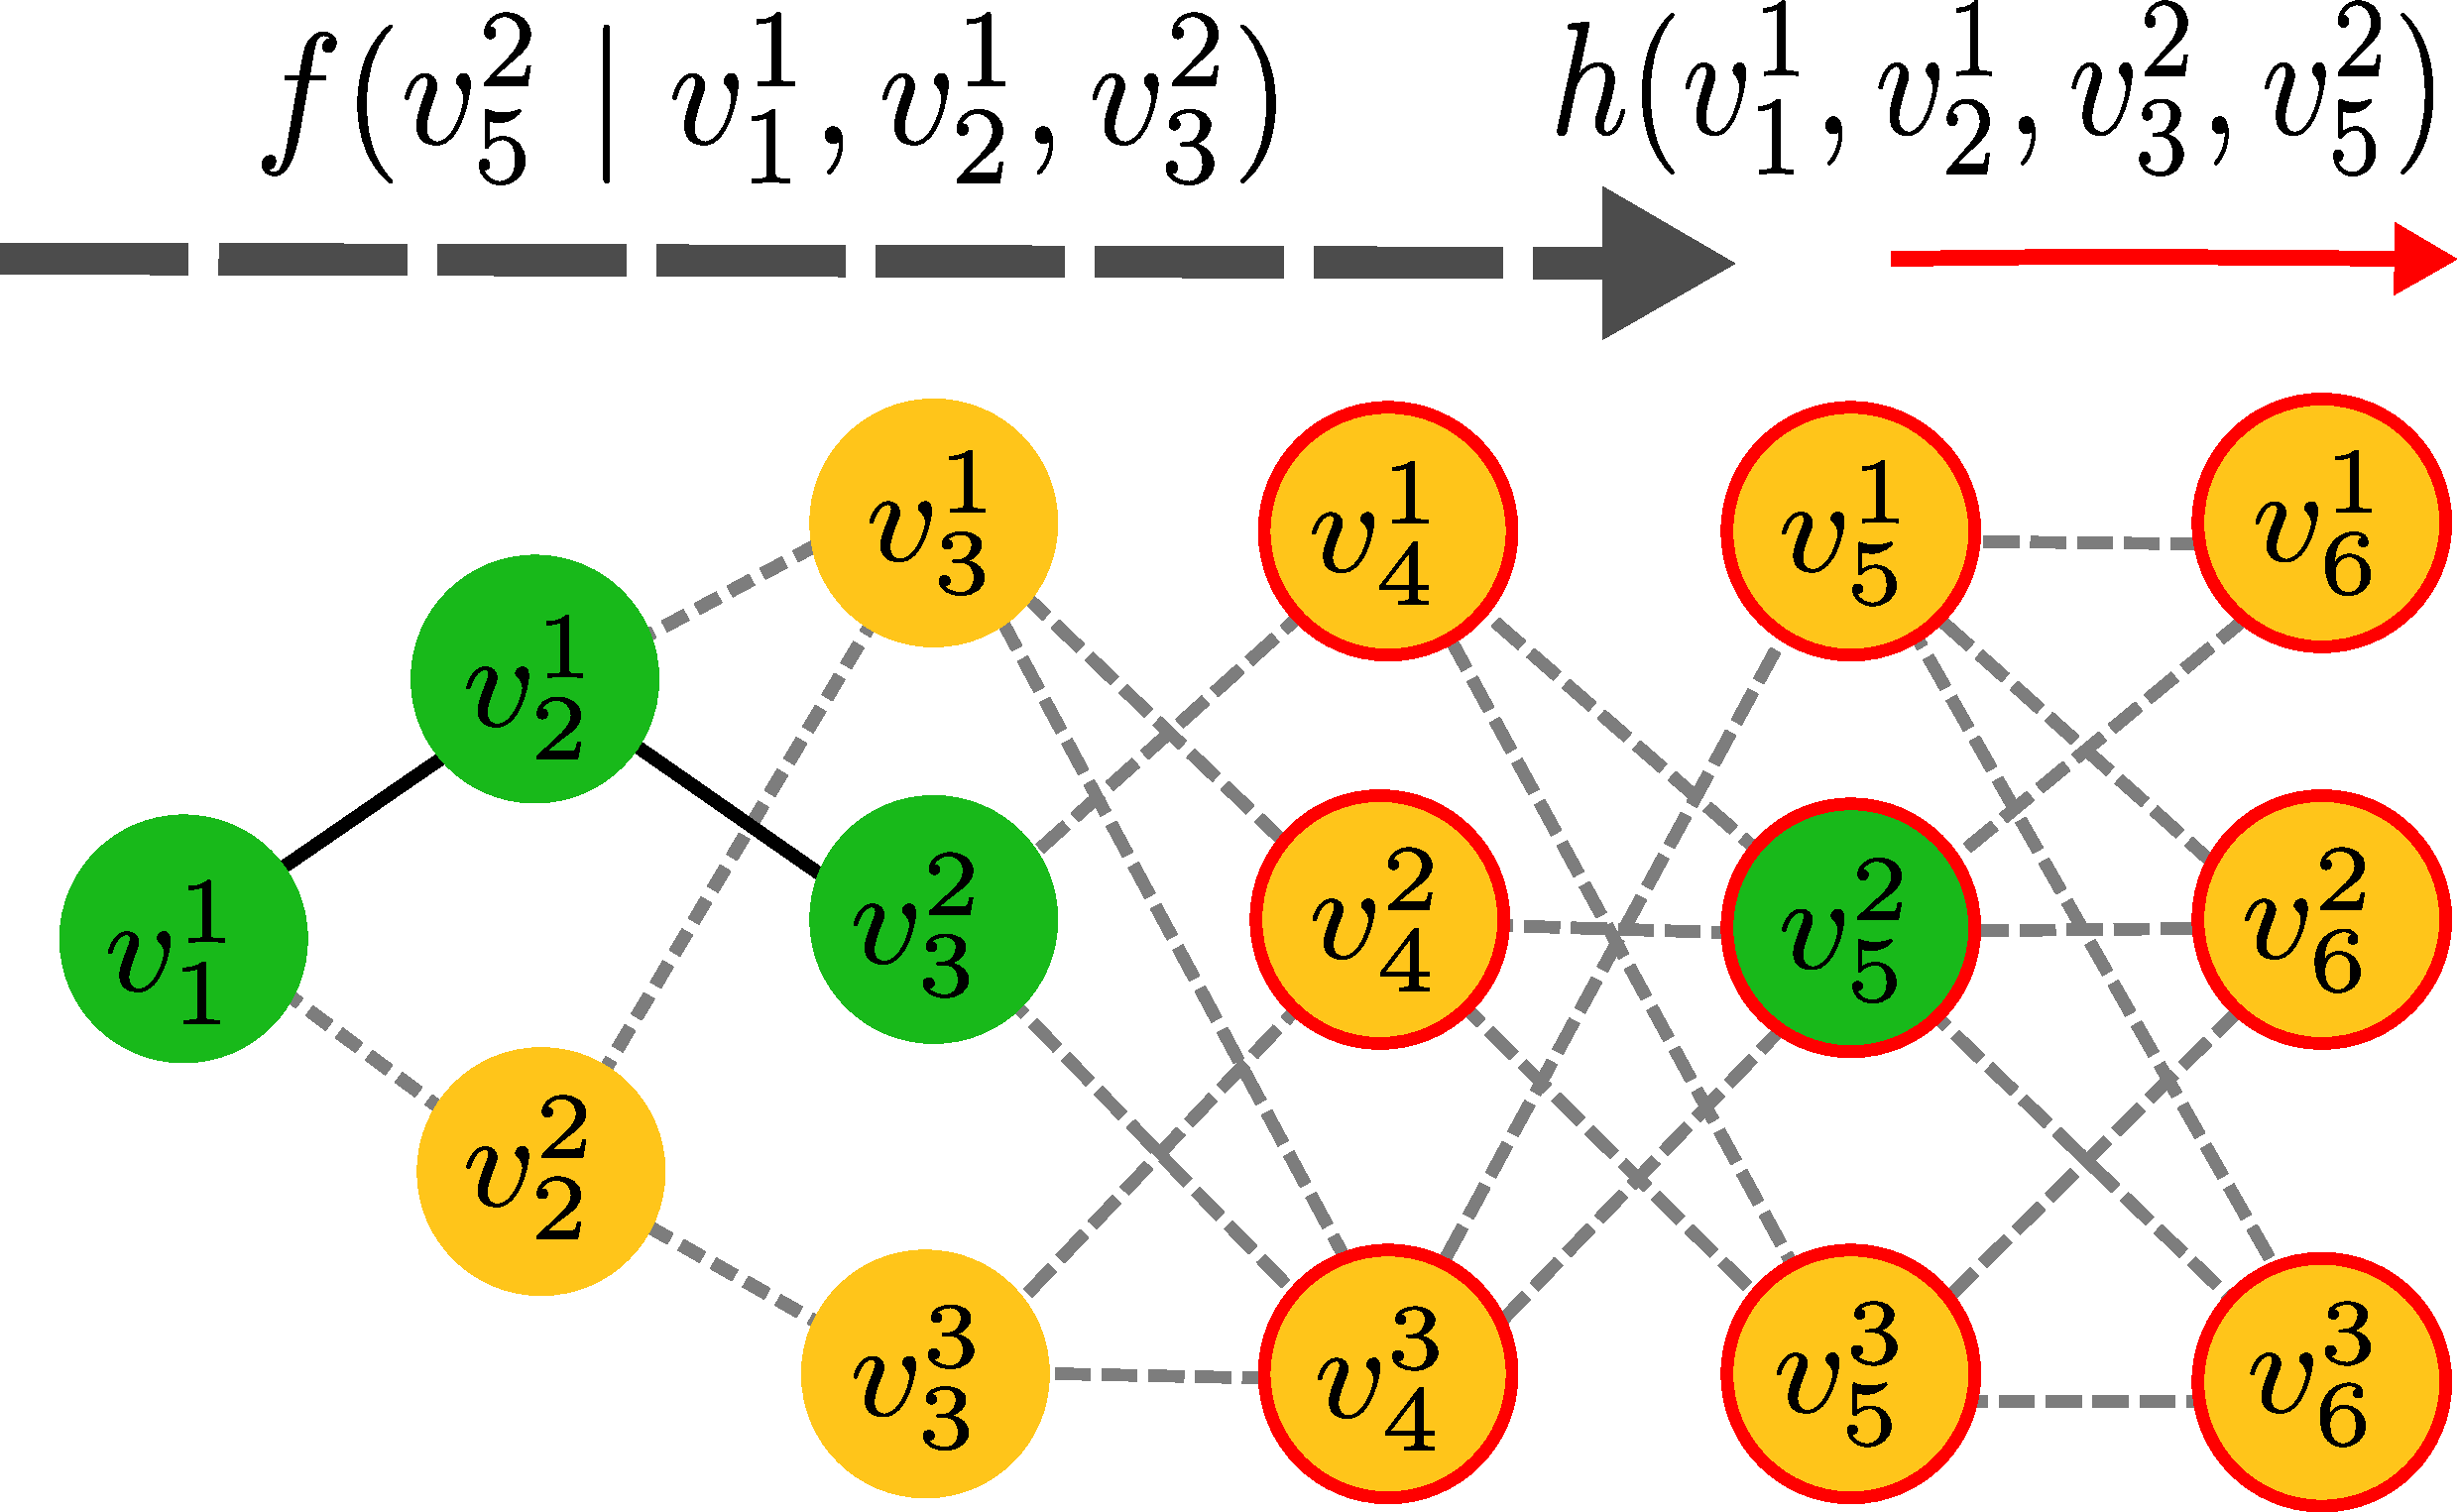
\includegraphics[width = 0.9\textwidth]{./figure/DefineFuncP}
\end{figure}
\end{block}
\end{columns}

\begin{figure}
\centering

\includegraphics[width = 0.9\textwidth]{./figure/DefineFuncHelp}
\end{figure}

\end{frame}

\begin{frame}{Backtracking}{Heuristic}

\begin{columns}

\column{0.6\textwidth}
\begin{minipage}{\textwidth}
\begin{figure}
\centering
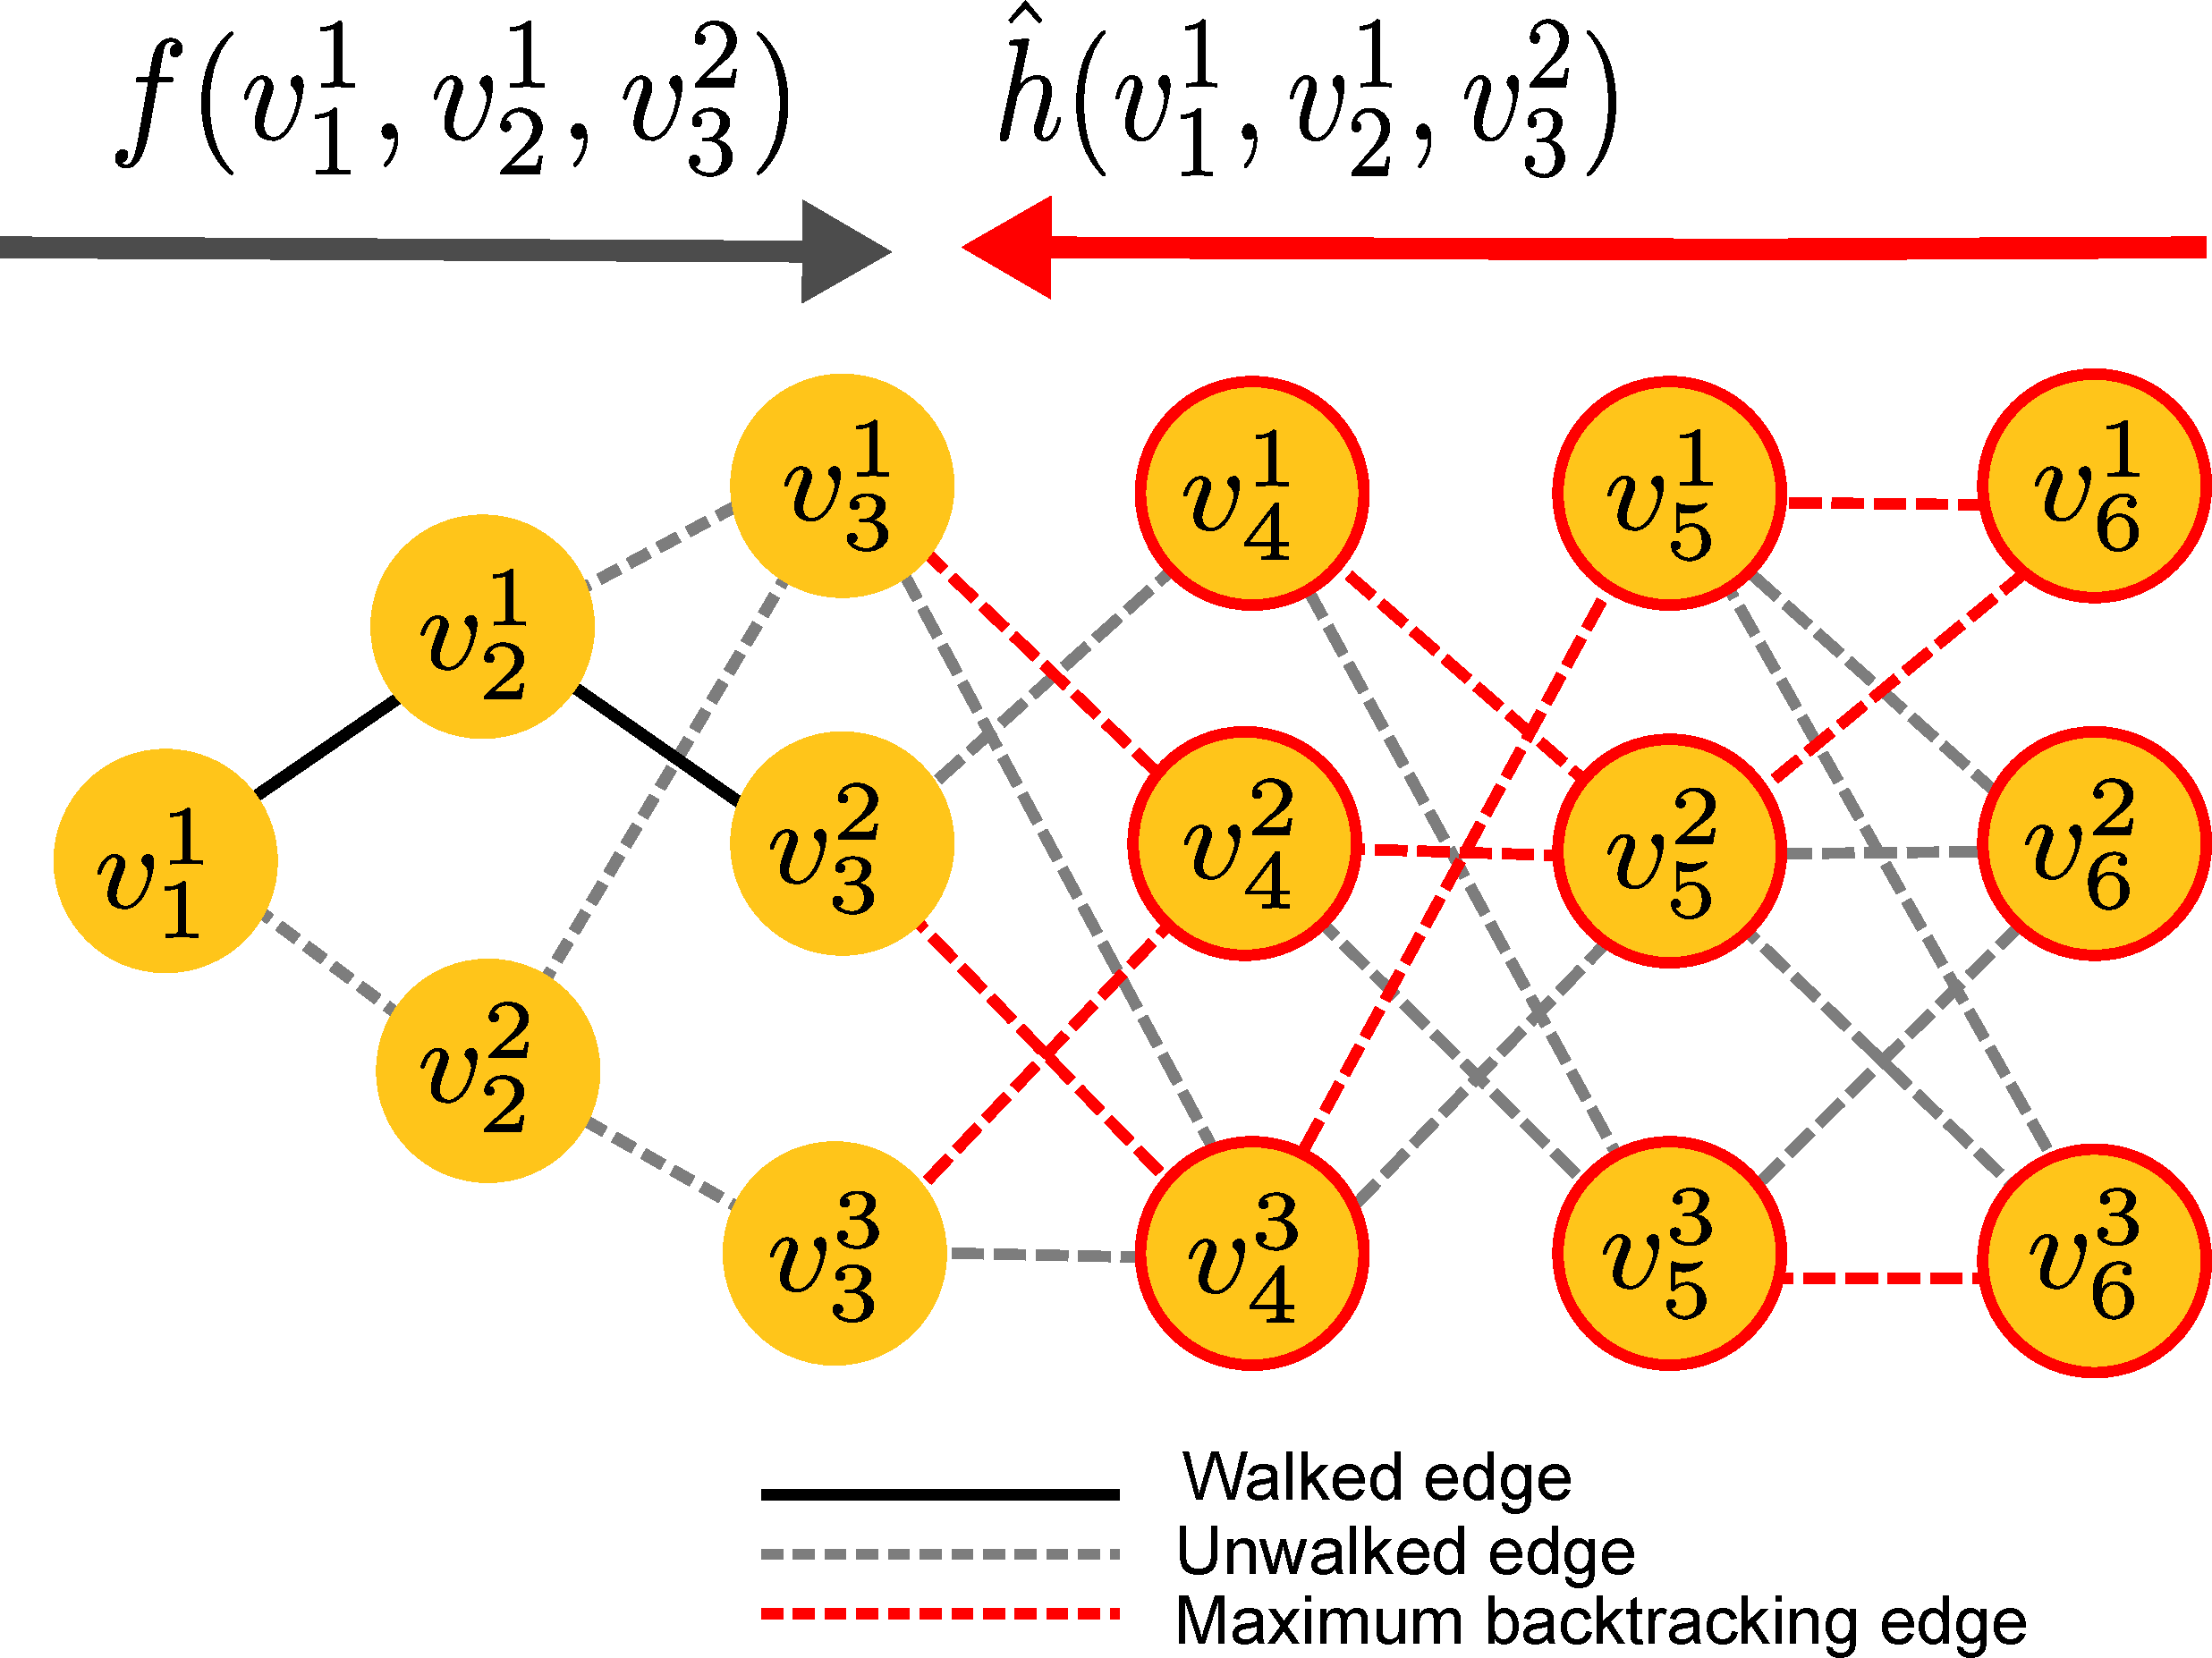
\includegraphics[width = \textwidth]{./figure/backtracking}
\end{figure}
\end{minipage}

\column{0.4\textwidth}
\begin{minipage}{\textwidth}
\begin{itemize}
\item point model $ \rightarrow $ true max total reward
\item coverage model $ \rightarrow $ estimated max total reward guarantee
\end{itemize}
\end{minipage}

\end{columns}

\end{frame}

\subsection{Anytime algorithm design}

\begin{frame}{Expanding tree}{Anytime algorithm framework}

\begin{columns}

\column{0.6\textwidth}
\begin{minipage}{\textwidth}
\begin{figure}
\centering
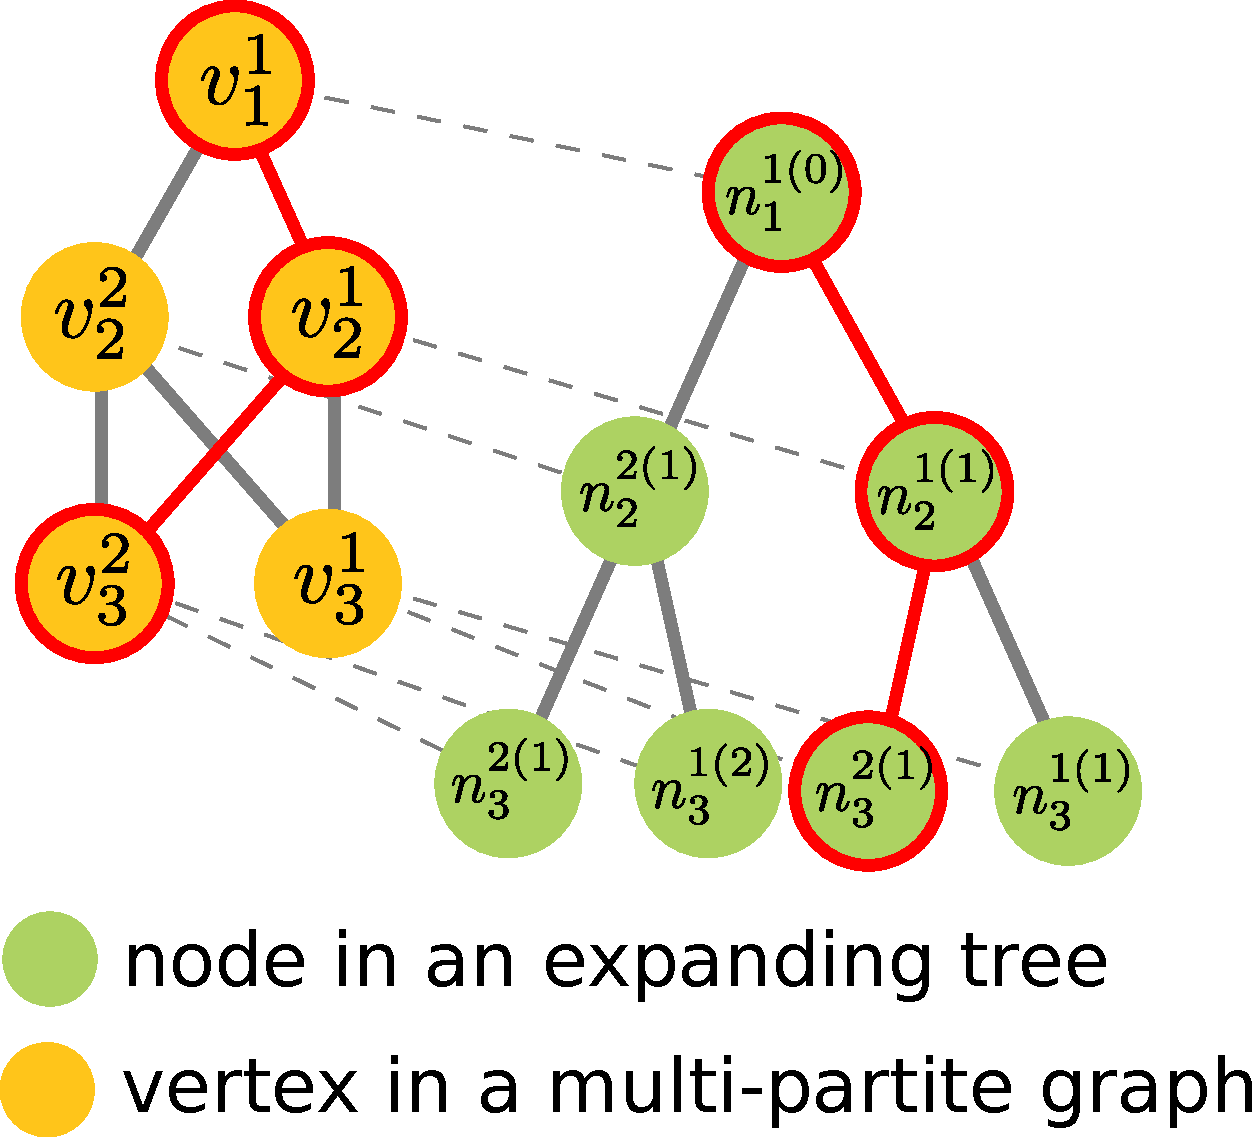
\includegraphics[width=.9\textwidth]{./figure/multipartite_expandingtree}
\end{figure}
\end{minipage}


\column{0.4\textwidth}
\begin{minipage}{\textwidth}

Exhaustive enumeration

\begin{itemize}
\item depth-first recursive traverse
\item node $ \Longleftrightarrow $ subpath
\end{itemize}
%Exapnding tree $ G_{T} = (N, L, T) $ \\
%\begin{itemize}
%\item $ T $ - tree depth
%\item $ N $ - Node set
%\item $ L $ - directed link set
%\end{itemize}
\end{minipage}

\end{columns}

\end{frame}

\begin{frame}{Expanding tree}{Anytime algorithm framework}

\begin{columns}

\column{0.6\textwidth}
\begin{minipage}{\textwidth}
\begin{figure}
\centering
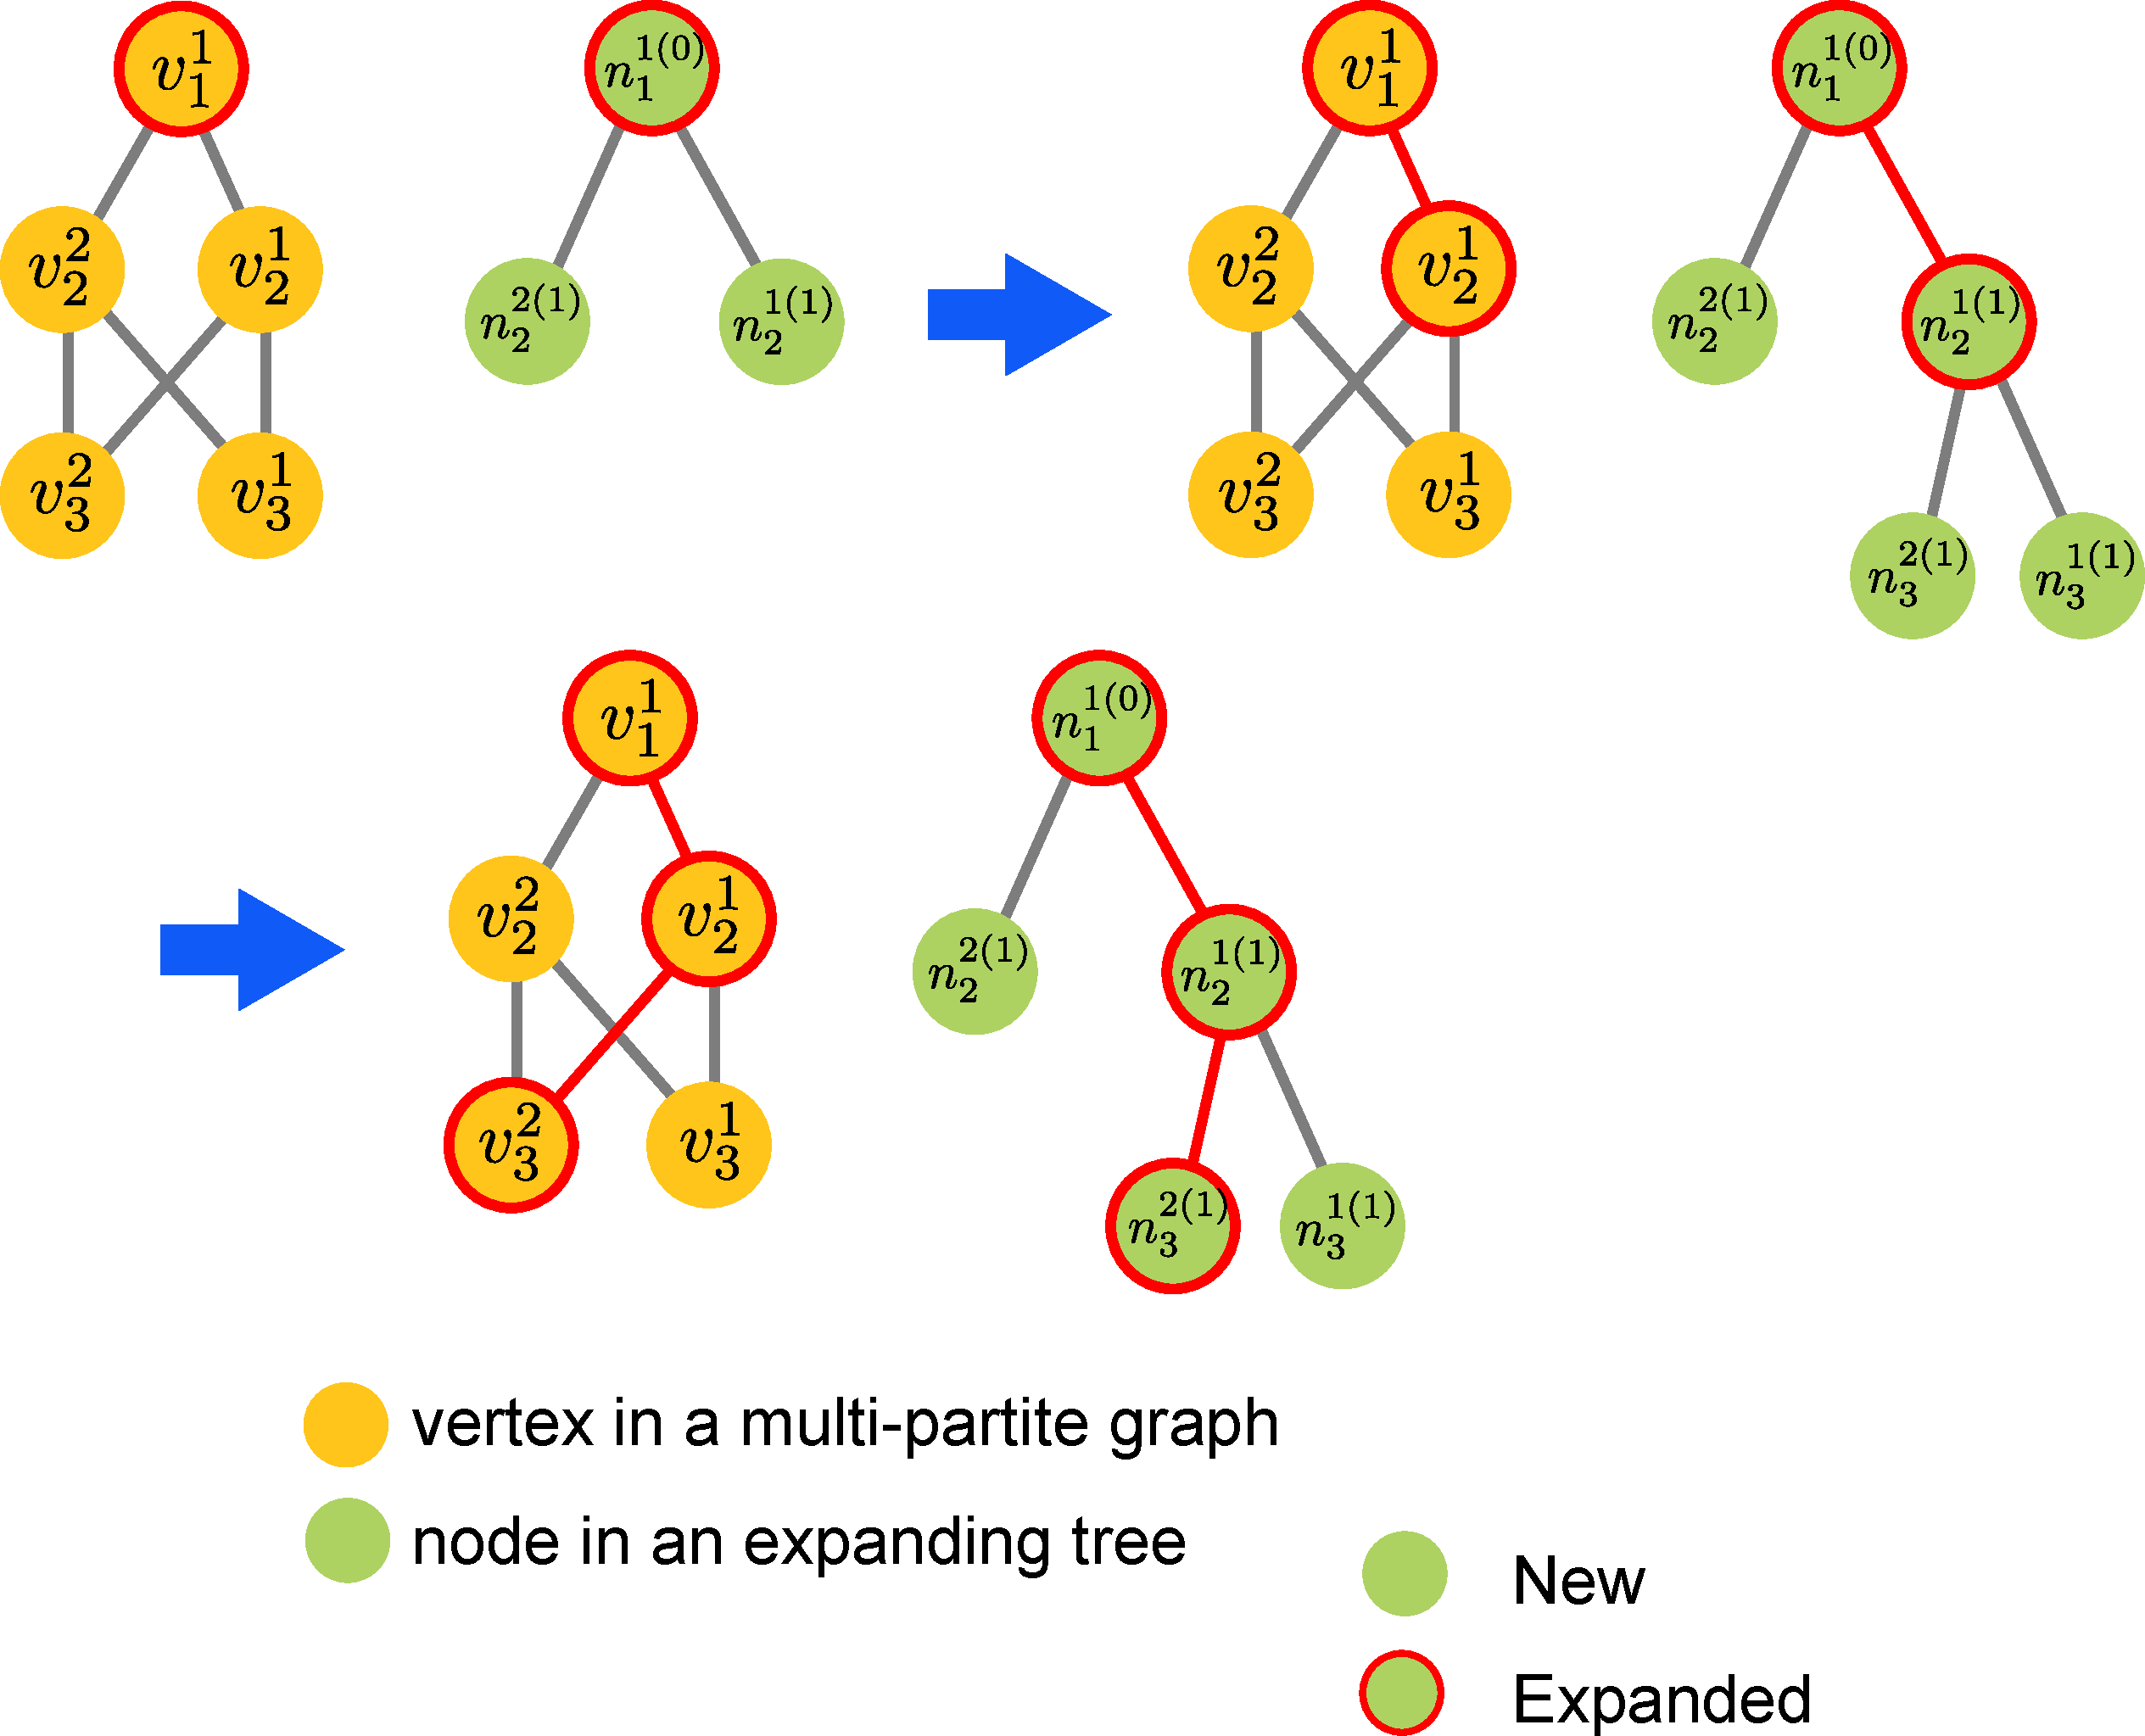
\includegraphics[width=\textwidth]{./figure/tree_expanding_process}
\end{figure}
\end{minipage}


\column{0.4\textwidth}
\begin{minipage}{\textwidth}

Tree expanding

\begin{itemize}
\item tracking the search process
\item estimation storage
\end{itemize}
%Exapnding tree $ G_{T} = (N, L, T) $ \\
%\begin{itemize}
%\item $ T $ - tree depth
%\item $ N $ - Node set
%\item $ L $ - directed link set
%\end{itemize}
\end{minipage}

\end{columns}

\end{frame}

\begin{frame}{Node freeze}{Anytime algorithm framework}

%node cannot be possible to yield better path than best path we already found, there is no reason to explore this

Estimated reward $ \leq $ Current best reward 
$ \Longrightarrow $ Stop exploring subpath

\begin{figure}
\centering
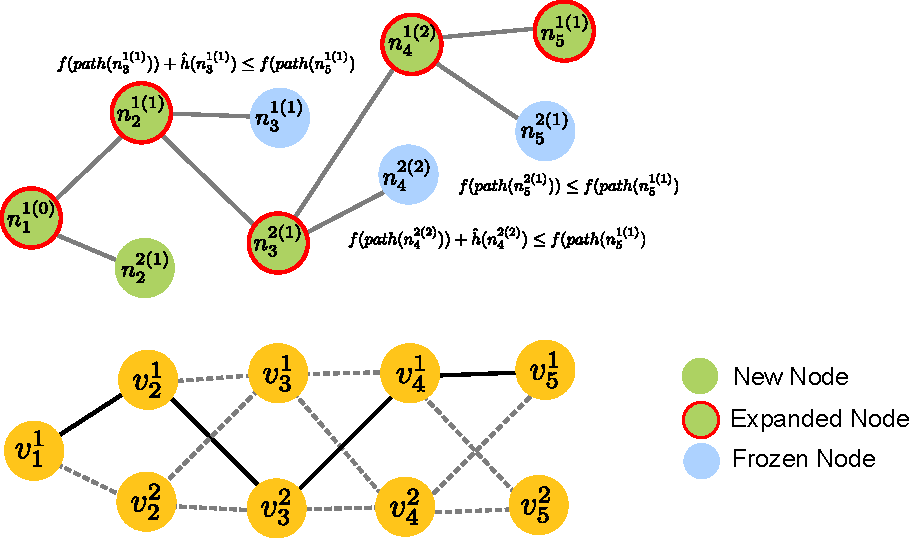
\includegraphics[width =  0.8\textwidth]{./figure/freeze_process}
\end{figure}

\end{frame}

\begin{frame}{Flow}{Anytime algorithm framework}

\begin{figure}
\centering
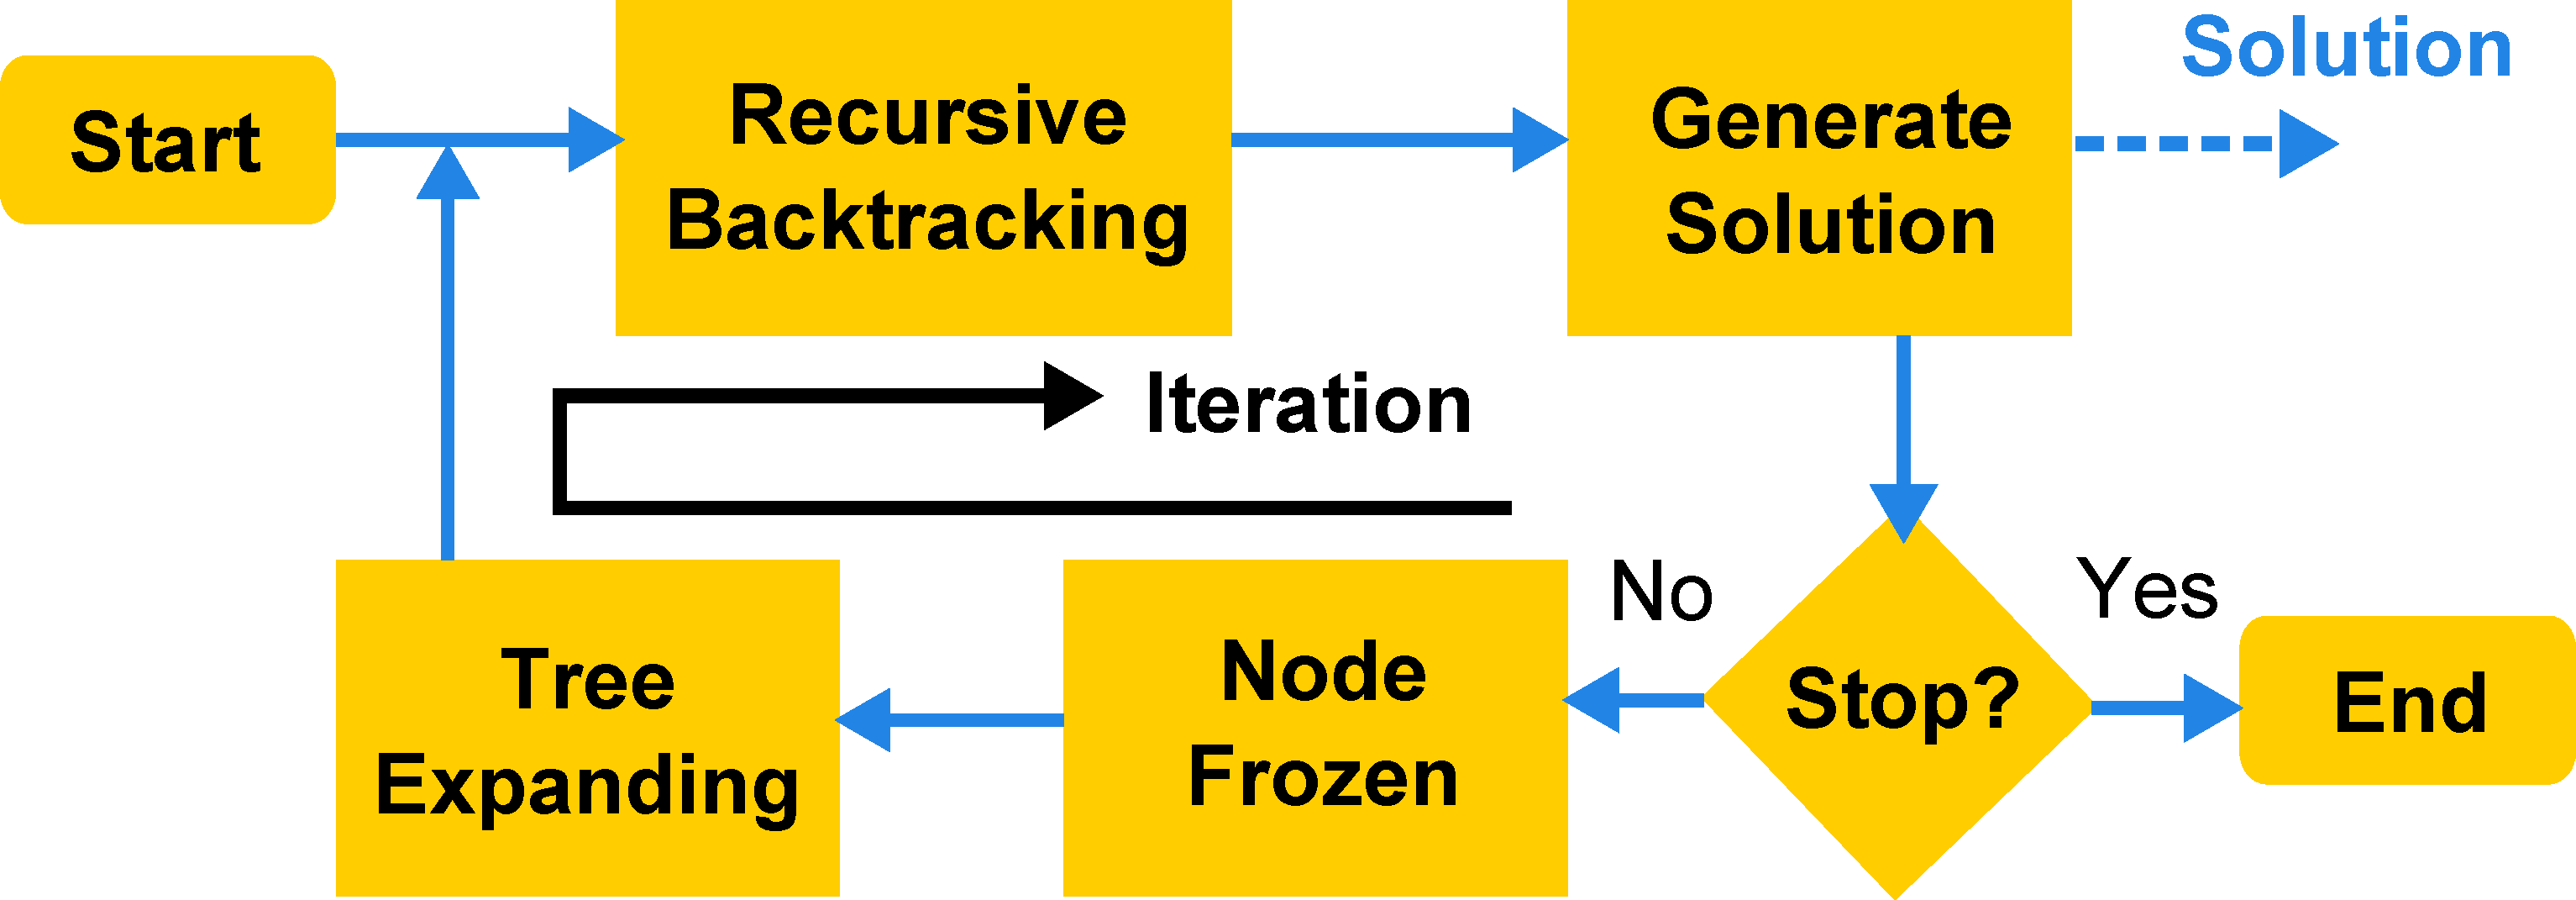
\includegraphics[width = 0.9\textwidth]{./figure/alg_flow}
\end{figure}

\end{frame}

\begin{frame}{Performance guarantee}{Anytime algorithm framework}

\begin{lemma}
“Backtracking” in Algorithm 1 never \textcolor{red}{underestimates}
the maximum total reward, which means
\begin{equation}
\nonumber
\forall t \geq t', \hat{u}(x_{t} \mid v_{1} , \cdots , v_{t'}) \geq u(x_{t} \mid v_{1} , \cdots , v_{t'}).
\end{equation}
\end{lemma}

\begin{minipage}{\textwidth}
\begin{figure}
\centering

\includegraphics[width = 0.15\textwidth]{./figure/arrow}
\end{figure}
\end{minipage}

\begin{theorem}
The anytime algorithm framework in Algorithm 4 can always find an \textcolor{red}{optimal} solution given enough time.
\end{theorem}

\end{frame}